% ============================================================================
% Draft appendix: uncertainty of the network model.
% Written to be \input into the JHEP paper (jheppub), after \appendix.
% Comments beginning with "% TODO" mark decisions or numbers to revisit.
% Figures: fig_app_accuracy.pdf, fig_app_calibration.pdf,
%          fig_app_decomposition.pdf. References: appendix_refs.bib.
% Draft of 1 November 2026, v2: stage-1 (L1) ensembles only; the fine-tune
% version is kept in v1_finetune/.
% ============================================================================
\section{Uncertainty of the network model}
\label{app:uncertainty}

The differential cross section is modelled as
$\sigma(m_{hh},\theta) = \sum_{i=1}^{23} c_i(\theta)\, a_i(m_{hh})$, where the
monomials $c_i(\theta)$ in the HEFT parameters
$\theta = (\kappa_\lambda, c_t, c_{tt}, c_{ggh}, c_{gghh})$ are known
exactly~\cite{Alasfar:2023xpc} and the 23 functions $a_i(m_{hh})$ are represented by a
neural network (section~\ref{sec:model}). % TODO: label of the main-text section
In this appendix we describe how the network is trained, how its uncertainty is
estimated, and how both are validated on POWHEG spectra not used in the training.

\subsection{Data and noise model}
\label{app:data}

The training sample consists of 3,989 POWHEG spectra at 13~TeV, each at a different point
$\theta$, binned in 80 bins of 15~GeV between $m_{hh} = 255$ and 1455~GeV. Each bin of
each spectrum is one training row, $(m_{hh}, \theta) \mapsto \sigma$. Of the 317,306 rows,
274,152 are used for training, 5,078 for validation (the choice of the saved parameters),
and 38,076 are not used in the training. A further 1,000 spectra, generated in the same
way, are held out completely and serve as the test sample.

Every spectrum is, to a good approximation, a histogram of $N_\text{eff}$ events of equal
weight. We estimate $N_\text{eff}$ from the bin-to-bin fluctuations of the training
spectra in the smooth region $m_{hh} > 570$~GeV, comparing each bin with the average of its
two neighbours, and find $N_\text{eff} \simeq 3.8 \times 10^4$. The noise variance of bin
$k$ of a spectrum with total cross section $\sigma_\text{tot}$ is then taken to be
\begin{equation}
  \sigma_k^2 = \Big(t_k + \frac{\sigma_\text{tot}}{N_\text{eff}}\Big)
               \frac{\sigma_\text{tot}}{N_\text{eff}} ,
  \label{eq:app:noise}
\end{equation}
where $t_k$ is the POWHEG cross section in the bin; the second term, the variance of one
additional event, prevents bins with very few events from acquiring unphysically small
variances. Eq.~(\ref{eq:app:noise}) is used for the Bayesian network (appendix~\ref{app:bnn}); for
the test sample we use $\sigma_k^2 = t_k \sigma_\text{tot}/N_\text{eff}$.
% TODO: the per-spectrum event weights can be recovered exactly from the quantization
% of the spectra; a later version could use them instead of N_eff.

\subsection{Training}
\label{app:training}

Each network is trained by minimising the mean absolute deviation (L1 loss) between
prediction and POWHEG, with the Adam optimiser~\cite{Kingma:2014vow}, mini-batches of 2,048
rows, $2 \times 10^5$ iterations and a learning rate of $2 \times 10^{-3}$ halved three
times at equal intervals. The parameters with the lowest validation loss are kept. The L1
loss treats an absolute error equally in every bin, so the fit is dominated by the largest
cross sections, and the region just above threshold, where the cross section is two orders
of magnitude below its peak, is modelled less precisely (table~\ref{tab:app:accuracy}).
% TODO: one sentence on the fine-tune with a Huber loss of the pulls (threshold chi2 per
% bin 4.1 -> 1.6, but then a model-error term is needed); see v1_finetune/.

\subsection{Ensembles}
\label{app:ensembles}

We regard the training procedure as an estimator $\hat f(\boldsymbol{x}; D, s)$ of the
cross section at $\boldsymbol{x} = (m_{hh}, \theta)$, which depends on the training sample
$D$ and on a random seed $s$ that fixes the initial weights and the order of the
mini-batches. Its standard deviation at fixed $\boldsymbol{x}$ is the standard error of the
network prediction. We estimate it with a \emph{bootstrap}
ensemble~\cite{Efron:1979,Efron:1993} of $M = 20$ networks: member $m$ is trained, with
seed $s = 42 + m$, on 274,152 rows drawn with replacement from the training rows (on
average 63\% distinct). The ensemble mean $\bar f$ is the prediction and the standard
deviation $s$ of the members its uncertainty; with $M = 20$, $s$ is itself uncertain by
about 16\%.

The bootstrap treats the training rows as independent draws from a population of rows and
estimates the variability of the result under a repetition of the whole procedure with a
new sample of the same size. This is one of several defensible reference ensembles: one
could instead resample whole spectra (new points $\theta$) or regenerate the POWHEG events
at fixed $\theta$; the choice is not dictated by the data~\cite{Freedman:1981,Davison:1997}.
% TODO: optional sentence on the reference-class problem (Venn, Fisher, Cox 1958).

To identify the source of the spread we also trained a \emph{seeds} ensemble: the same 20
seeds, all on the original training rows. Because member $m$ uses the same seed in both
ensembles, the law of total variance,
\begin{equation}
  \operatorname{Var}_{D,s}[\hat f] =
  \operatorname{E}_D\big[\operatorname{Var}_s[\hat f \mid D]\big]
  + \operatorname{Var}_D\big[\operatorname{E}_s[\hat f \mid D]\big] ,
  \label{eq:app:totvar}
\end{equation}
separates the bootstrap variance (left) into an optimisation term, estimated by the seeds
ensemble, and a data term, their difference. Ensembles of independently trained networks
are known to capture the variability between equally good solutions (``deep
ensembles'')~\cite{Lakshminarayanan:2016,Wilson:2020}.

\subsection{Bayesian cross-check}
\label{app:bnn}

As a cross-check we sampled the posterior density of the 3,944 network parameters
following Neal~\cite{Neal:1996}, with Hamiltonian Monte Carlo~\cite{Duane:1987,Neal:2011},
using a hierarchical Gaussian prior with one Gibbs-sampled precision per parameter tensor
and a Gaussian likelihood with the known variances~(\ref{eq:app:noise}). The step size and
a diagonal mass matrix were adapted during a warm-up of $10^3$
iterations~\cite{Hoffman:2014}, after which $10^3$ samples were drawn with 800 leapfrog
steps per trajectory, starting from a network trained as in appendix~\ref{app:training}.
The effective sample size of the predictions at the monitored points is about 135.
Because the likelihood weights each bin by its precision, the posterior mean is more
accurate than the ensemble mean near threshold (table~\ref{tab:app:accuracy}); elsewhere
the two agree, differing by a median of 0.8 ensemble standard deviations. The posterior
standard deviation, however, is only 0.5\% of the POWHEG noise: with
$2.7 \times 10^5$ training rows the parameters of a single network are tightly
constrained, and the posterior describes neither the variability between equally good
networks, which a single Markov chain does not explore, nor the model's own error. We
therefore do not use it as the uncertainty.

\subsection{Validation on the test spectra}
\label{app:validation}

On the 1,000 test spectra we compute, for every bin, the $\chi^2$ contribution
$(t_k - \bar f_k)^2/\sigma_k^2$ and the pull
\begin{equation}
  z_k = \frac{t_k - \bar f_k}{\sqrt{\sigma_k^2 + s_k^2}} .
  \label{eq:app:pull}
\end{equation}
If $s_k$ accounts for the difference between the network and the true cross section, $z$
has unit standard deviation. Table~\ref{tab:app:accuracy} and figure~\ref{fig:app:accuracy}
show the accuracy, table~\ref{tab:app:calibration} and figure~\ref{fig:app:calibration} the
calibration, and figure~\ref{fig:app:decomposition} the decomposition~(\ref{eq:app:totvar}).
% TODO: update all numbers below after the re-run of the bootstrap ensemble.

\begin{table}[t]
\centering
\small
\begin{tabular}{lccccc}
\hline
 & median $\chi^2/N$ & $\chi^2/N > 5$ & \multicolumn{2}{c}{$\langle\chi^2\rangle$ per bin} & negative \\
 & & & 255--555 GeV & $> 555$ GeV & predictions \\
\hline
single network & 1.171 & 4.9\% & 8.44 & 1.20 & 0.18\% \\
bootstrap ensemble & 1.118 & 2.2\% & 4.05 & 1.14 & 0.06\% \\
seeds ensemble & 1.127 & 2.3\% & 4.08 & 1.17 & 0.06\% \\
Bayesian network (posterior mean) & 1.099 & 1.2\% & 1.89 & 1.12 & 0.03\% \\
\hline
\end{tabular}
\caption{Accuracy on the 1,000 test spectra. $\chi^2/N$ is computed per spectrum; the
columns give its median and the fraction of spectra above 5, and the mean $\chi^2$ per bin
below and above 555~GeV. For the ensembles, the mean of the 20 members is used.}
\label{tab:app:accuracy}
\end{table}

\begin{figure}[t]
\centering
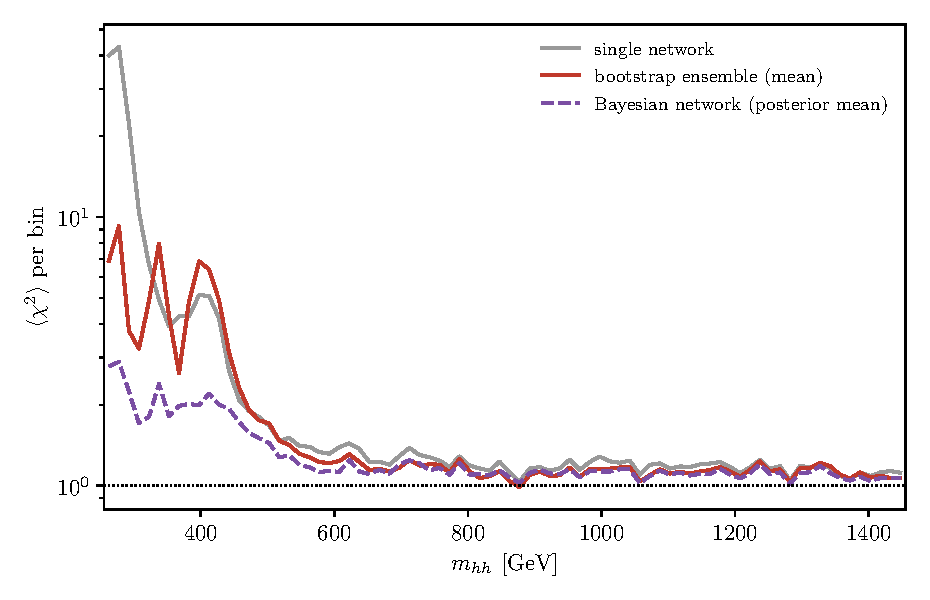
\includegraphics[width=0.7\textwidth]{fig_app_accuracy.pdf}
\caption{Mean $\chi^2$ per bin over the 1,000 test spectra as a function of $m_{hh}$, for a
single network, the mean of the bootstrap ensemble, and the posterior mean of the Bayesian
network.}
\label{fig:app:accuracy}
\end{figure}

\paragraph{Accuracy.} Averaging over the ensemble improves on a single network everywhere,
and most just above threshold, where the mean $\chi^2$ per bin falls from 8.4 to 4.1; the
members differ most there (their individual values range from 3.6 to 15). Above 555~GeV
the ensemble mean is within 15\% of the POWHEG noise level ($\langle\chi^2\rangle = 1.14$).
Negative predictions, which are unphysical, become rare.

\begin{table}[t]
\centering
\small
\begin{tabular}{lcccccc}
\hline
 & \multicolumn{2}{c}{median $s/\sigma_k$} & \multicolumn{3}{c}{standard deviation of $z$} & $|z| < 2$ \\
 & all & 255--555 GeV & all & 255--555 GeV & $> 555$ GeV & \\
\hline
bootstrap ensemble & 0.157 & 0.25 & 1.025 & 1.020 & 1.026 & 95.0\% \\
seeds ensemble & 0.157 & 0.25 & 1.024 & 1.018 & 1.026 & 95.0\% \\
Bayesian network & 0.005 & 0.007 & 1.143 & 1.370 & 1.055 & 93.5\% \\
\hline
\end{tabular}
\caption{Calibration on the test spectra: the uncertainty $s$ in units of the POWHEG noise,
and the pull~(\ref{eq:app:pull}). For a standard normal pull, $|z| < 2$ holds for 95.4\% of
bins.}
\label{tab:app:calibration}
\end{table}

\begin{figure}[t]
\centering
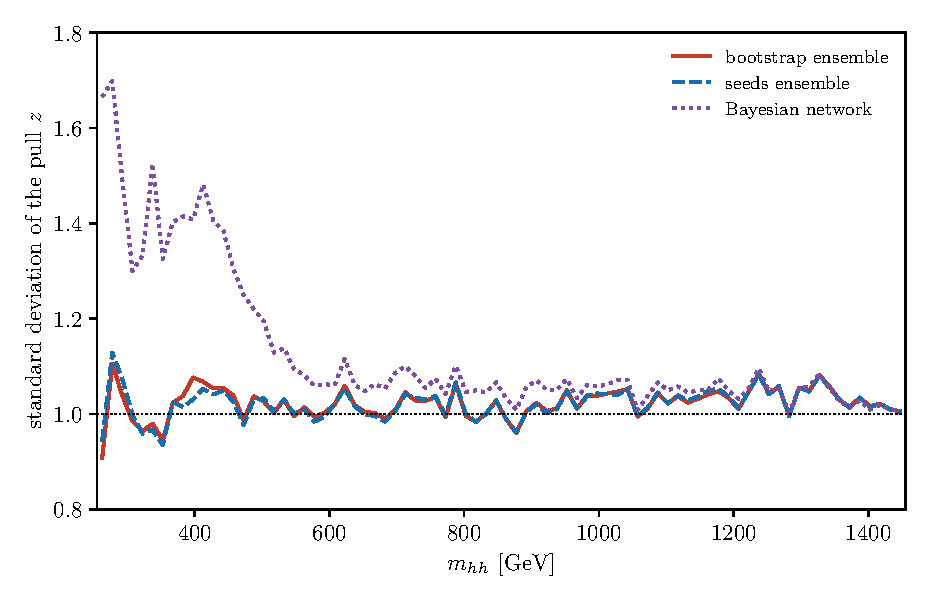
\includegraphics[width=0.7\textwidth]{fig_app_calibration.pdf}
\caption{Standard deviation of the pull~(\ref{eq:app:pull}) as a function of $m_{hh}$.}
\label{fig:app:calibration}
\end{figure}

\paragraph{Calibration.} The spread of the ensemble matches its error: the pull has unit
standard deviation within 2--3\% at all $m_{hh}$, including the threshold region, where
both the error of the mean and the disagreement between members are largest. No additional
model-error term is needed. The tails of the pull distribution are somewhat heavier than
Gaussian: 0.56\% of bins have $|z| > 3$, against 0.27\% for a standard normal. The Bayesian
posterior is far too narrow, as explained in appendix~\ref{app:bnn}.

\begin{figure}[t]
\centering
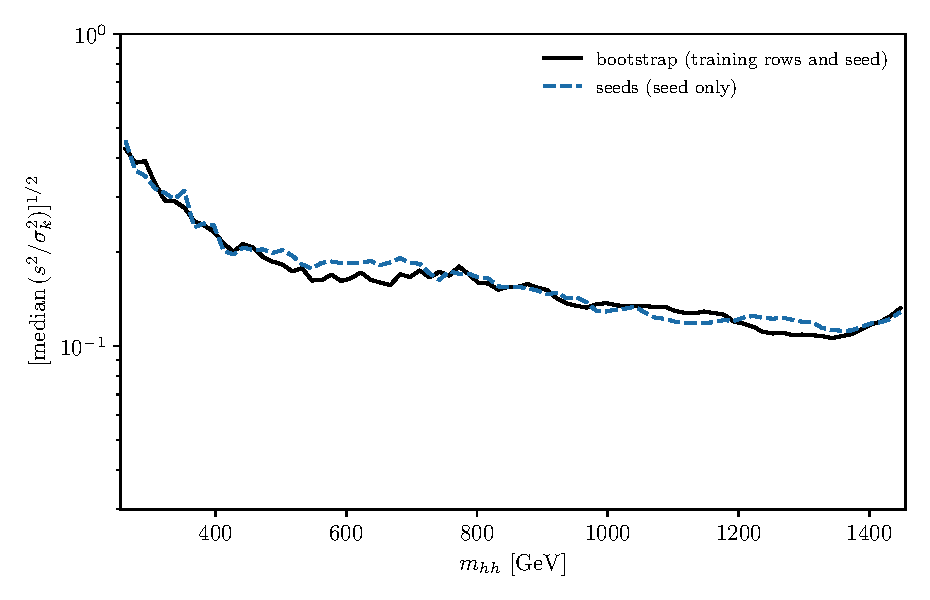
\includegraphics[width=0.7\textwidth]{fig_app_decomposition.pdf}
\caption{Spread of the bootstrap ensemble (training rows and seed varied) and of the seeds
ensemble (seed varied only), as the square root of the median over the test spectra of
$s^2/\sigma_k^2$.}
\label{fig:app:decomposition}
\end{figure}

\paragraph{Sources of the spread.} The bootstrap and seeds variances are equal within the
statistical uncertainty of 20-member ensembles (figure~\ref{fig:app:decomposition}; the
median ratio of the seeds to the bootstrap variance is 1.05), and the means of the two
ensembles agree to 0.2 of their spread. The spread is therefore due almost entirely to the
optimisation, i.e.\ to the different, equally good solutions reached from different
starting points; the variability due to the finite training sample is too small to be
measured with these ensembles. % TODO: if the re-run gives a smaller ratio, quote it here
% (e.g. "about 80% of the variance is due to the seed").

\subsection{Summary}
\label{app:summary}

The cross-section model used in this paper is the mean of a bootstrap ensemble of 20
networks trained with an L1 loss, and its uncertainty is the standard deviation of the
members. On 1,000 independent POWHEG spectra this model reaches a median $\chi^2/N$ of
1.12, and its uncertainty is calibrated to within 3\% at all $m_{hh}$. The uncertainty is
dominated by the variability between equally good networks, which is largest just above
threshold; the variability due to the finite training sample is negligible in comparison.
A Bayesian treatment of the network parameters gives a compatible central value, but its
posterior width is negligible and does not describe the uncertainty of the model.
